\chapter{Entscheidungssysteme}
\label{chap:entscheidungssysteme}

Die Entscheidungsfindung ist die Entscheidung, welche Aktionen f\"{u}r einen NPC gew\"{a}hlt werden. Sie wird \"{u}ber sogenannte Entscheidungssysteme realisiert. Basierend auf dem Zustand des NPC, f\"{u}hren sie verschiedene Aktionen \"{u}ber Komponenten, welche im Kapitel \ref{chap:komponenten} erläutert werden, durch. Nach dem Fund der jeweiligen Aktion gibt der Prozessor dem Entscheidungssystem Zeit, die dazugeh\"{o}rige Komponente auszuf\"{u}hren. In diesem Kapitel werden die verschiedenen Arten von Entscheidungssystemen in den Bereichen Game-AI und Robotik vorgestellt.

\section{Ad-Hoc Behavioring Authoring}
\label{chap:ahba}

Zu den popul\"{a}rsten Entscheidungssystemen der Game-AI geh\"{o}ren die Ad-Hoc Behaviour Authoring Methoden. Zu diesen geh\"{o}ren die FSMs und BTs. Die Ad-Hoc Behaviour Authoring Methoden dominieren die Entscheidungsfindung der NPCs in der Game-AI. Bei den Methoden wird die Verhaltensweise der NPCs explizit programmiert. Sie beinhalten normalerweise keine Art von Algorithmen zum Lernen oder Suchen von Entscheidungen. Sie sind leicht zu implementieren, visualisieren und debuggen. Mit der steigenden Komplexit\"{a}t der NPCs wird es jedoch schwieriger, das Entscheidungssystem zu designen, erweitern oder anzupassen. \autocite{aiag, review_game_ai}

\subsection{Finite State Machine}
\label{chap:fsm}

Die FSM wird als Graph repr\"{a}sentiert. Die FSM speichert dabei Informationen in Knoten, die wiederum Kanten besitzen, die zu weiteren Knoten f\"{u}hren. Eine FSM kann sich zu jedem Zeitpunkt nur in einem Knoten befinden. Ein Knotenwechsel erfolgt, wenn die Bedingung f\"{u}r die entsprechende Kante erf\"{u}llt ist. 

In der Game-AI repr\"{a}sentieren die Knoten die Zust\"{a}nde des NPC, wie zum Beispiel das Patrouillieren oder Angreifen. Die Zust\"{a}nde der Knoten werden \"{u}ber Komponenten ausgef\"{u}hrt. So ben\"{o}tigt der Zustand des Patrouillierens solche Komponenten, die ihn zu bestimmten Punkten bewegen. Die \"{U}berg\"{a}nge \"{u}ber die Kanten zwischen den Zust\"{a}nden erfolgen \"{u}ber Bedingungen. So kann ein NPC vom Zustand des Patrouillierens in den des Angreifens wechseln, sobald die Bedingung erf\"{u}llt ist, dass der NPC den Spieler sieht. Die NPCs des FPS Half-Life wurde beispielsweise \"{u}ber eine FSM realisiert. \autocite{AIgames}

\begin{figure}[h]
  \centering
  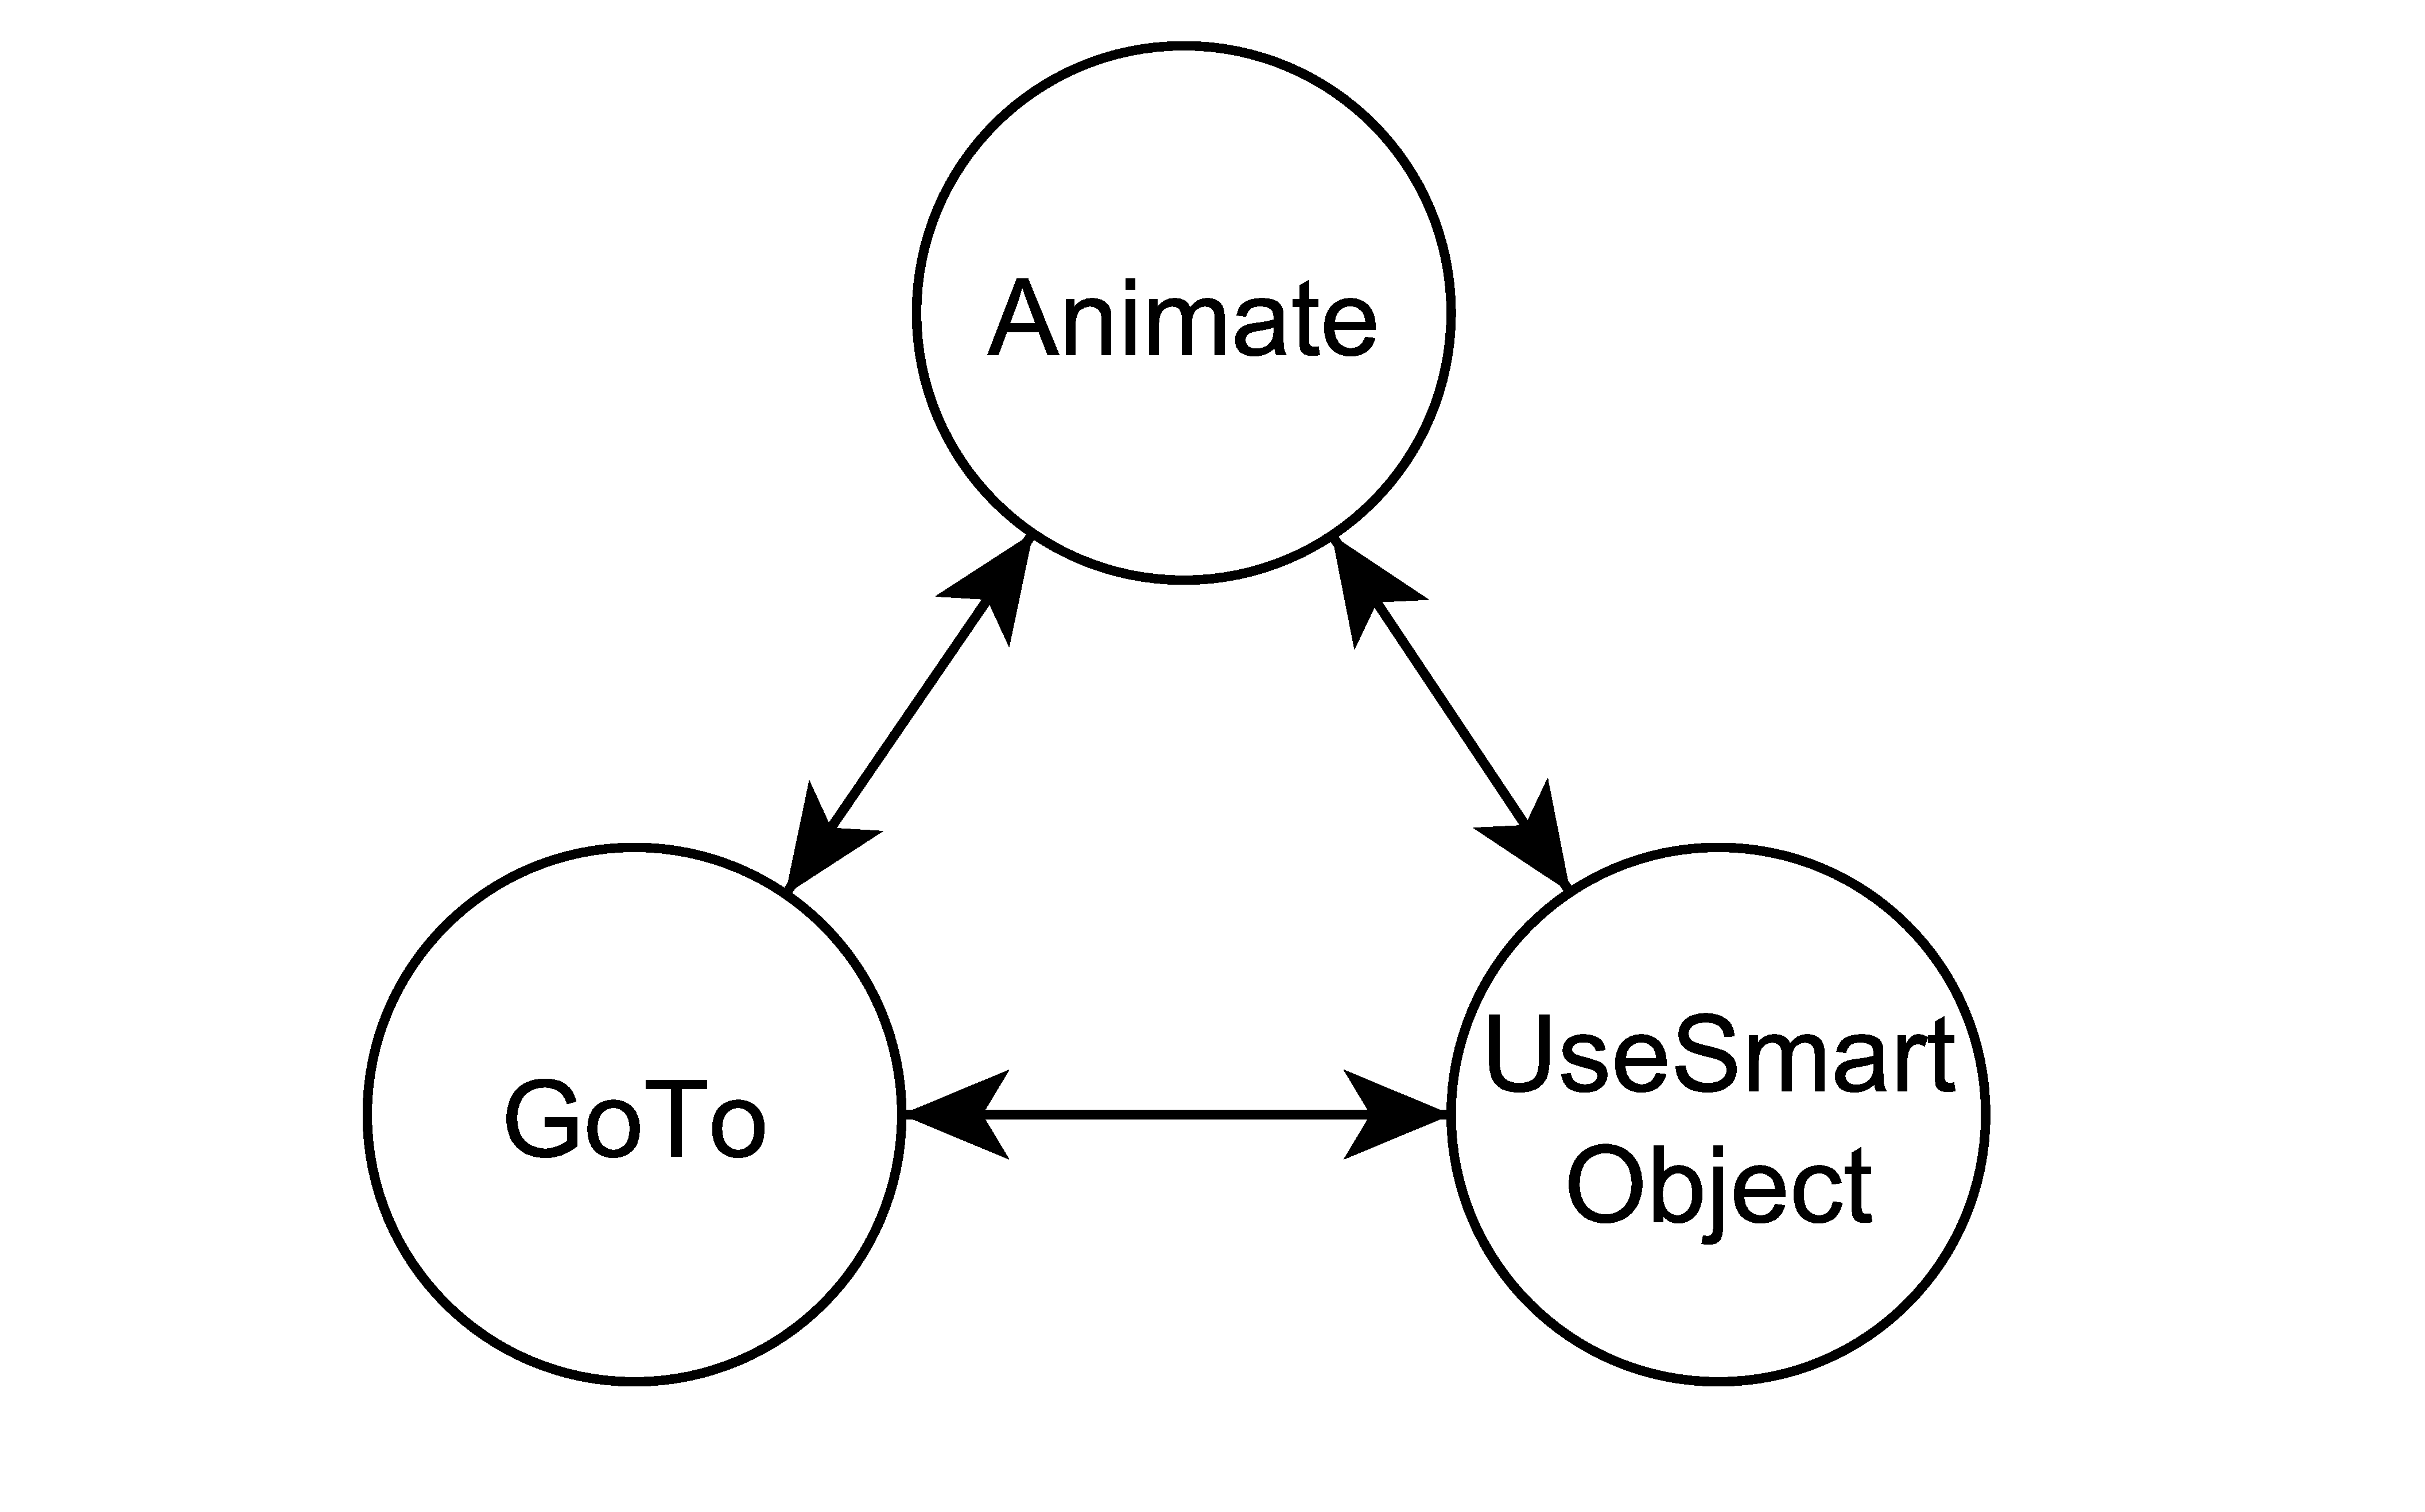
\includegraphics[width=\textwidth]{Entscheidungssysteme/fsm}
	\captionsetup{justification=justified, format=plain}
  \caption{Finite State Machine Beispiel}
  \label{fig:ES FSM}
\end{figure}


\subsection{Behavior Tree}
\label{chap:bt}

Der BT wird als Baumstruktur dargestellt. Anders als die FSM besitzt der BT keine Zust\"{a}nde, sondern Tasks. Diese Tasks lassen sich in verschiedene Kategorien einteilen und erhalten \"{u}ber den Prozessor Zeit, ihr Skript durchzuf\"{u}hren.

% Run, Success oder Failure gro\ss{} klein?
Nach der Ausf\"{u}hrung gibt das Skript des Tasks einen der folgenden Werte zur\"{u}ck: Run, Success oder Failure. Run impliziert, dass der Task noch aktiv ist, Success, dass der Task erfolgreich abgeschlossen wurde und Failure, dass der Task fehlgeschlagen ist. Bei jedem Ausf\"{u}hrung f\"{u}hrt ein BT eine Tiefensuche durch, bis ein niedrigstufiges Task Blatt entweder Success oder Run zur\"{u}ckgibt \autocite{qlbt}.

Die Kategorien der Tasks lauten wie folgt: Conditions, Actions und Composites. Die Condition Task pr\"{u}ft Bedingungen, die einen Wert wie Success oder Failure zur\"{u}ckgibt, wie zum Beispiel, ob der Spieler zu sehen ist. Meistens findet die Ausf\"{u}hrung der Condition Task vor der Action Task statt. Die Action Taks f\"{u}hrt anschlie\ss{}end ihre Aktion \"{u}ber Komponenten des NPC durch, wie zum Beispiel zu schie\ss{}en oder in Deckung zu gehen. Beide Task Kategorien sind die Bl\"{a}tter der Baumstruktur.

Die dritte Kategorie ist die Composite Task, welche die Sammlung der Child-Tasks, also der Condition- und Action-Tasks, verwaltet. Das Verhalten der Composite Task basiert auf dem resultierenden Wert der Child-Tasks. Die Composite Task l\"{a}sst sich in zwei Subkategorien, Sequences und Selectors, aufteilen. Basierend auf dem R\"{u}ckgabewert wird entschieden, ob der n\"{a}chste Child-Task ausgef\"{u}hrt wird oder der Composite stoppt und selbst einen R\"{u}ckgabewert zur\"{u}ckgibt. So gibt ein Selector den R\"{u}ckgabewert Success, sobald einer seiner Child-Tasks Success zur\"{u}ckgibt. Sollte ein Child-Task dagegen Failure zur\"{u}ckgeben, so wird der n\"{a}chste Child-Task ausgef\"{u}hrt, bis keine Child-Tasks verf\"{u}gbar sind und der Selector folglich Failure an seinen Parent zur\"{u}ckgibt. So f\"{u}hren Selectors die erstm\"{o}gliche Child-Task in ihrem Set aus. Eine Sequence gibt Failure als R\"{u}ckgabewert, sobald einer seiner Child-Tasks Failure zur\"{u}ckgibt. Erst, wenn alle Child-Tasks Success zur\"{u}ckgeben, gibt die Sequence den R\"{u}ckgabewert Success zur\"{u}ck. Eine Sequence repr\"{a}sentiert ein Set an Aktionen, die durchgef\"{u}hrt werden m\"{u}ssen. Ein Beispiel f\"{u}r die Umsetzung des BT als Entscheidungssystem f\"{u}r NPCs ist der FPS Halo 2. \autocite{AIgames, review_game_ai}

\begin{figure}[h]
  \centering
  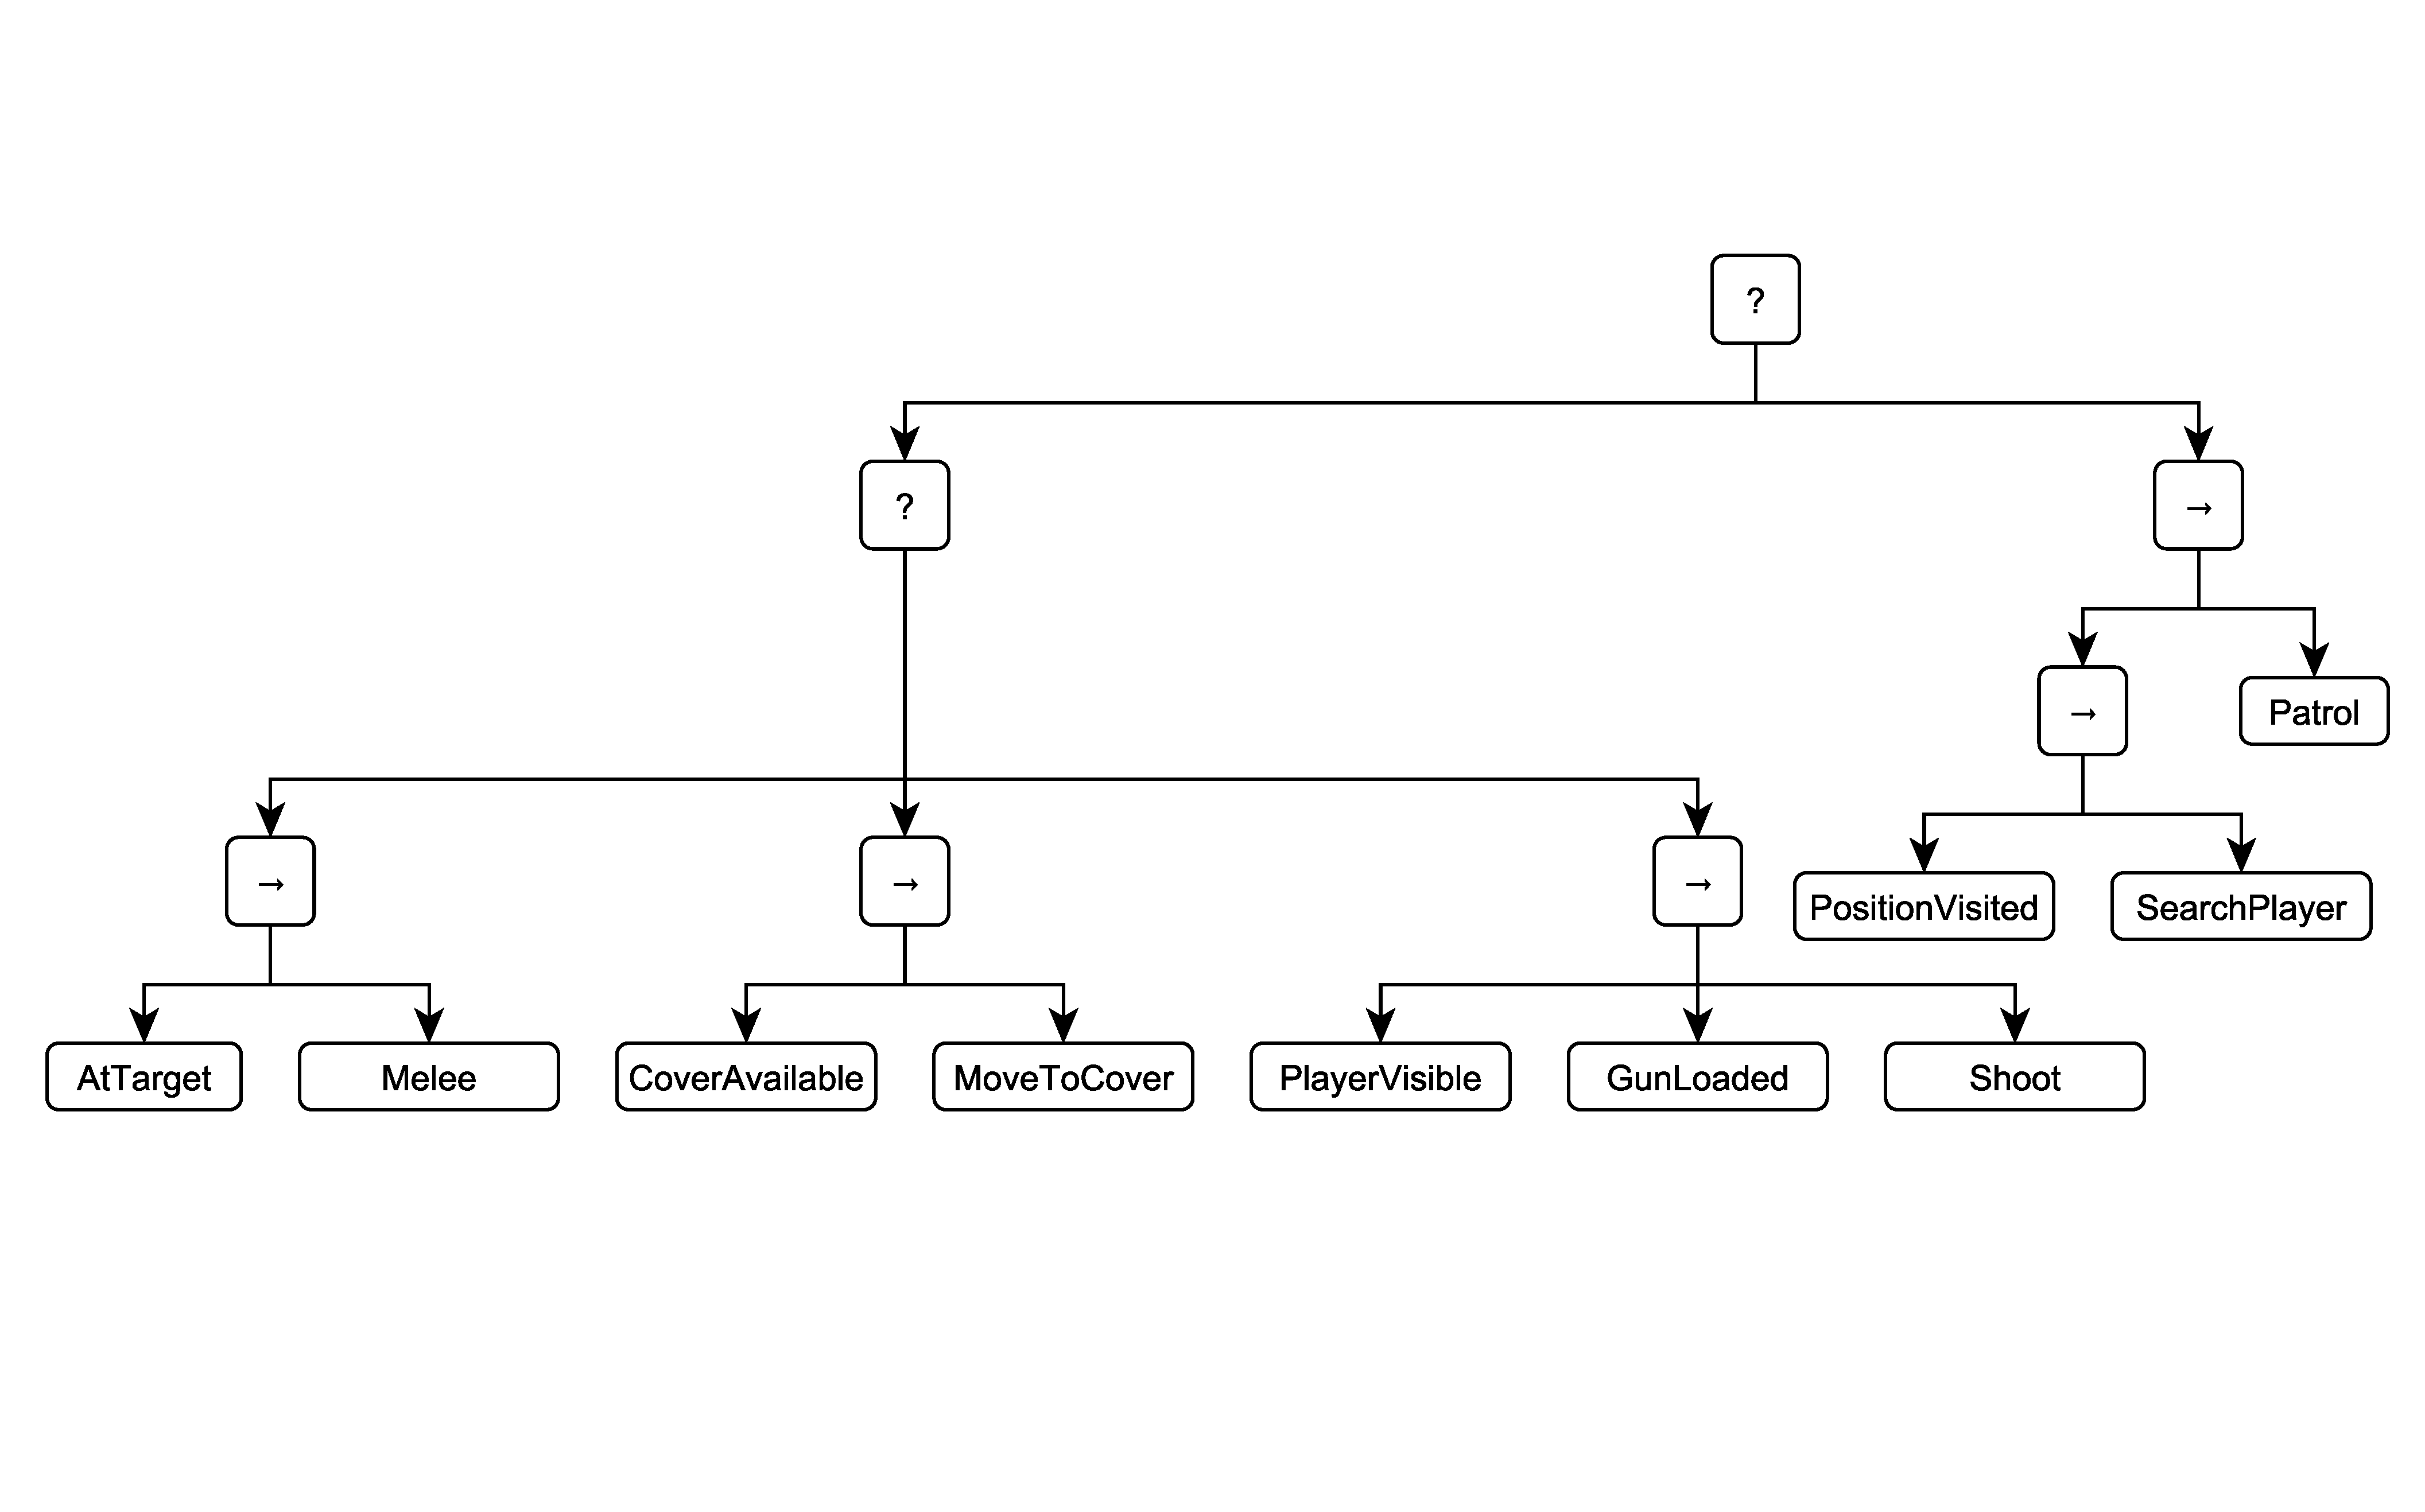
\includegraphics[width=\textwidth, trim=0cm 10cm 0cm 5cm, clip]{Entscheidungssysteme/behavior tree}
	\captionsetup{justification=justified, format=plain}
  \caption{Behavior Tree Beispiel an einem FPS-NPC}
  \label{BT}
\end{figure}


\section{Suchalgorithmen}
\label{chap:monte-carlo}

Aufgaben der AI k\"{o}nnen auch als Suchprobleme formuliert werden, die durch das Finden des besten Pfades gel\"{o}st werden. Die Suchalgorithmen konstruieren einen Suchbaum, bei dem der Wurzelknoten den Ausgangszustand darstellt, die Kanten die Operationen des Agenten repr\"{a}sentieren, die zu einem neuen Knoten f\"{u}hren, welcher einen neuen Zustand repr\"{a}sentiert. Aus einem Zustand sind mehrere Operationen m\"{o}glich. Einer der bekannteren Suchalgorithmen ist der Monte Carlo Tree Search (MCTS), welcher Bestandteil von AlphaGo ist \autocite{review_game_ai}. Ein weiterer bekannter Suchalgorithmus ist A*, welcher sowohl die Navigation der NPC als auch die Entscheidungsfindung in GOAP realisiert.

\section{Entscheidungssysteme in der Robotik}
\label{chap:robotik}

Entscheidungssysteme sind essenziell f\"{u}r autonome Roboter, da sie die Verarbeitung von Sensordaten, die Auswahl geeigneter Aktionen und die Anpassung an dynamische Umgebungen erm\"{o}glichen. In diesem Kapitel werden die Entscheidungssysteme FSM, BT sowie der Vorl\"{a}ufer von GOAP, der Stanford Research Institute Problem Solver (STRIPS), vorgestellt.

\subsection{Finite State Machine}
\label{chap:fsm robotik}

Bei der Entwicklung eines Roboter-Verhaltens wird darauf geachtet, dass die vielen Komponenten, die f\"{u}r das Verhalten n\"{o}tig sind, m\"{o}glichst effizient zusammenarbeiten. Eine der simpelsten Architekturen f\"{u}r die Umsetzung eines Roboter Verhaltens ist die FSM.

Ein Beispiel ist ein Linien-Folgender-Roboter, der mithilfe von FSM umsetzbar ist. Die FSM bestimmt die Aktion auf Basis des aktuellen Knotens des Roboters. Der Roboter kann seinen Knoten und damit seine Aktion wechseln. Wenn ein Sensor des Roboters beispielsweise erkennt, dass er sich nicht mehr innerhalb der schwarzen Linie bewegt, dann wechselt er in einen anderen Knoten, der durch seine Aktionen den Kurs des Roboters korrigiert. \autocite{balogh2019using}

\subsection{Behavior Tree}
\label{chap:bt robotik}

Der BT ist ein weiteres Entscheidungssystem in der Robotik und stammt urspr\"{u}nglich aus der Spielentwicklung. Wie auch die FSM, wird der BT f\"{u}r die Aufgabenorchestrierung eines Roboters eingesetzt. Im Vergleich zu der FSM ist der BT zwar komplexer umzusetzen, hat aber folgende Vorteile: Aktionen k\"{o}nnen im BT leichter wiederverwendet und erweitert werden. Zudem muss der BT nicht definieren, wie eine Aktion im Bezug zu einer nachfolgenden Aktion steht. \autocite{iovino2022survey}

Ein Konzept f\"{u}r die Nutzung eines BT in der Robotik ist die Umsetzung auf einem unbemannten Luftfahrzeug (UAV). Dabei kann der BT als Controller f\"{u}r einen Luftkampf dienen. \autocite{ogren2012increasing}

\subsection{Stanford Research Institute Problem Solver}
\label{chap:strips}

Zu dem Entscheidungssystem GOAP gibt es wenige Studien in dem Bereich der Robotik. Daraus l\"{a}sst sich schlie\ss{}en, dass der GOAP eine untergeordnete Rolle in der Robotik spielt. Der GOAP basiert auf dem \"{a}lteren Entscheidungssystem STRIPS, der wiederum im Roboter Shakey eingesetzt und in \autocite{nilsson1984shakey} dokumentiert wird.

Der STRIPS wurde erstmals f\"{u}r den mobilen Roboter mit dem Nicknamen Shakey als Plansystem f\"{u}r die Aktionen implementiert. Dieser Roboter wurde von 1966 bis 1972 als wissenschaftliches Projekt im Labor f\"{u}r k\"{u}nstliche Intelligenz des Stanford Research Institutes entwickelt. Das Ziel dieses Projekts war es, Konzepte und Techniken der k\"{u}nstlichen Intelligenz zu entwickeln. Diese Konzepte sollen Automaten erm\"{o}glichen, in realistischen Umgebungen unabh\"{a}ngig zu agieren. Insbesondere boten sie den Kontext und die Motivation f\"{u}r die Entwicklung des A*-Suchalgorithmus. Der Roboter konnte nach seiner Fertigstellung in R\"{a}umen fahren, Hindernisse und \"{A}nderungen in der Umgebung erkennen sowie Boxen verschieben. Gab man dem Roboter ein Ziel als logische-Formel, so sollte der STRIPS eine g\"{u}ltige Sequenz an solchen Aktionen zur\"{u}ckgeben, die nach ihrer Ausf\"{u}hrung das Ziel erreichen sollen.

Der STRIPS besteht aus den folgenden Modulen: Einen Ausgangszustand, gegebenen Zielzustand und eine Sammlung an Aktionen.

Der Ausgangszustand repr\"{a}sentiert das derzeitige Wissen \"{u}ber die Welt des Agenten, also seinen Status. Im Falle von Shakey k\"{o}nne es sich um die Position handeln, in der sich der Roboter befindet und das Wissen \"{u}ber seine Umwelt, wie zum Beispiel die Verbindung der R\"{a}ume.

Die Aktionen haben Effekte und Vorbedingungen. Die Vorbedingungen einer Aktion entscheiden, ob es m\"{o}glich ist, diese in die Sequenz aufzunehmen. Die Effekte werden \"{u}ber eine Add- und Delete-List realisiert. W\"{a}hrend die Delete-List Wissen \"{u}ber Zust\"{a}nde l\"{o}scht, f\"{u}gt die Add-List neues Wissen \"{u}ber Zust\"{a}nde hinzu. Durch die Durchf\"{u}hrung der Add- und Delete-List werden Zust\"{a}nde, wie der Ausgangszustand, ge\"{a}ndert.

Der Zielzustand wurde im Falle von Shakey durch die logische-Formel von dem Benutzer gegeben. STRIPS baut aus dem Ausgangszustand eine Sequenz an Aktionen, die daraufhin in ihrer Reihenfolge ausgef\"{u}hrt werden. Die Ausf\"{u}hrung der Aktionen und ihrer Effekte soll den Ausgangszustand so ver\"{a}ndern, dass der Agent zu seinem Zielzustand kommt.
